
\section{Background \& Problem}

All Open Container Initiative (OCI) compliant containers, including Kubernetes,
enforce CPU reservations using \cgroups{}' weight interface~\cite{oci-cgroups,
docker-docs-cgroups, container-isolation-article}, as do VM frameworks,
including Firecracker and
libvirt~\cite{firecracker-cgroups,afaas,libvirt-cgroups}. Kubernetes creates one
group for all BE services, given the lowest weight 1, all others are in separate
groups with higher weights (in our experiment the server requests 4 CPUs,
Kubernetes assigns it weight 157).

\begin{figure}[t]
    \centering
    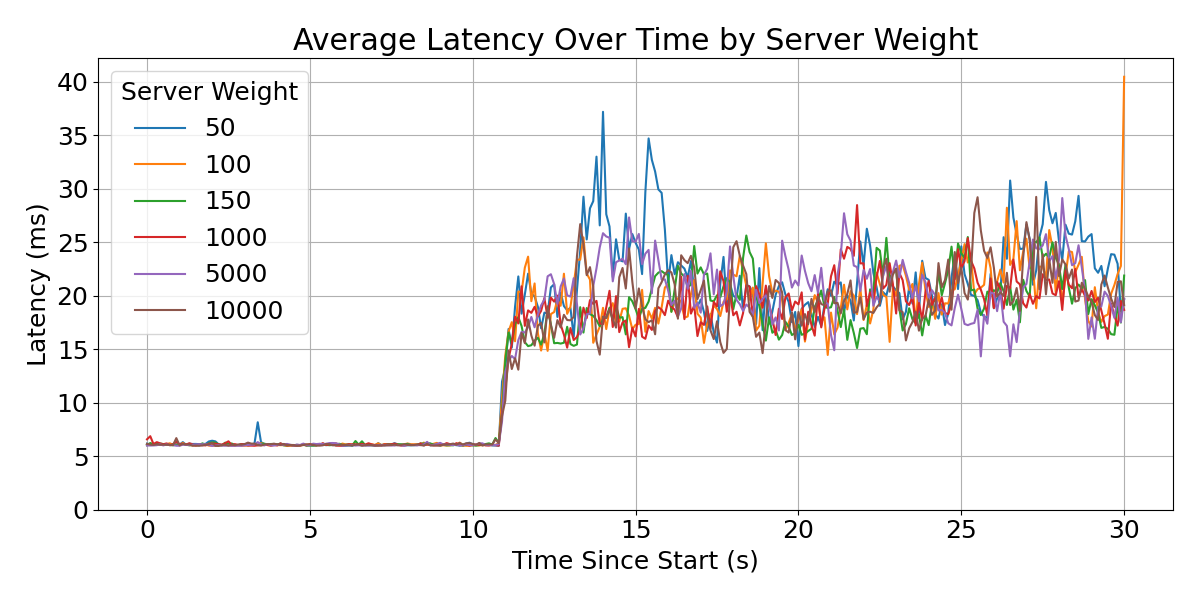
\includegraphics[width=\columnwidth]{graphs/srv-bg-weight-cmp-low.png}
    \caption{ the weight of the server has little impact on how much the
    weight 1 BE task interferes }\label{fig:srv-bg-weight-cmp}
\end{figure}


A simplified experiment shows \cgroups{} weights are unable to enforce
reservations. We run an open-loop remote client, with a simple LC CPU-bound
server and BE image resize job sharing four cores, each in their own group.
\cgroups{} supports weights in the range of [1,10000],
\autoref{fig:srv-bg-weight-cmp} shows that running the server with different
weights has no effect on the latency impact of the BE task.

\begin{figure}[t]
    \centering
    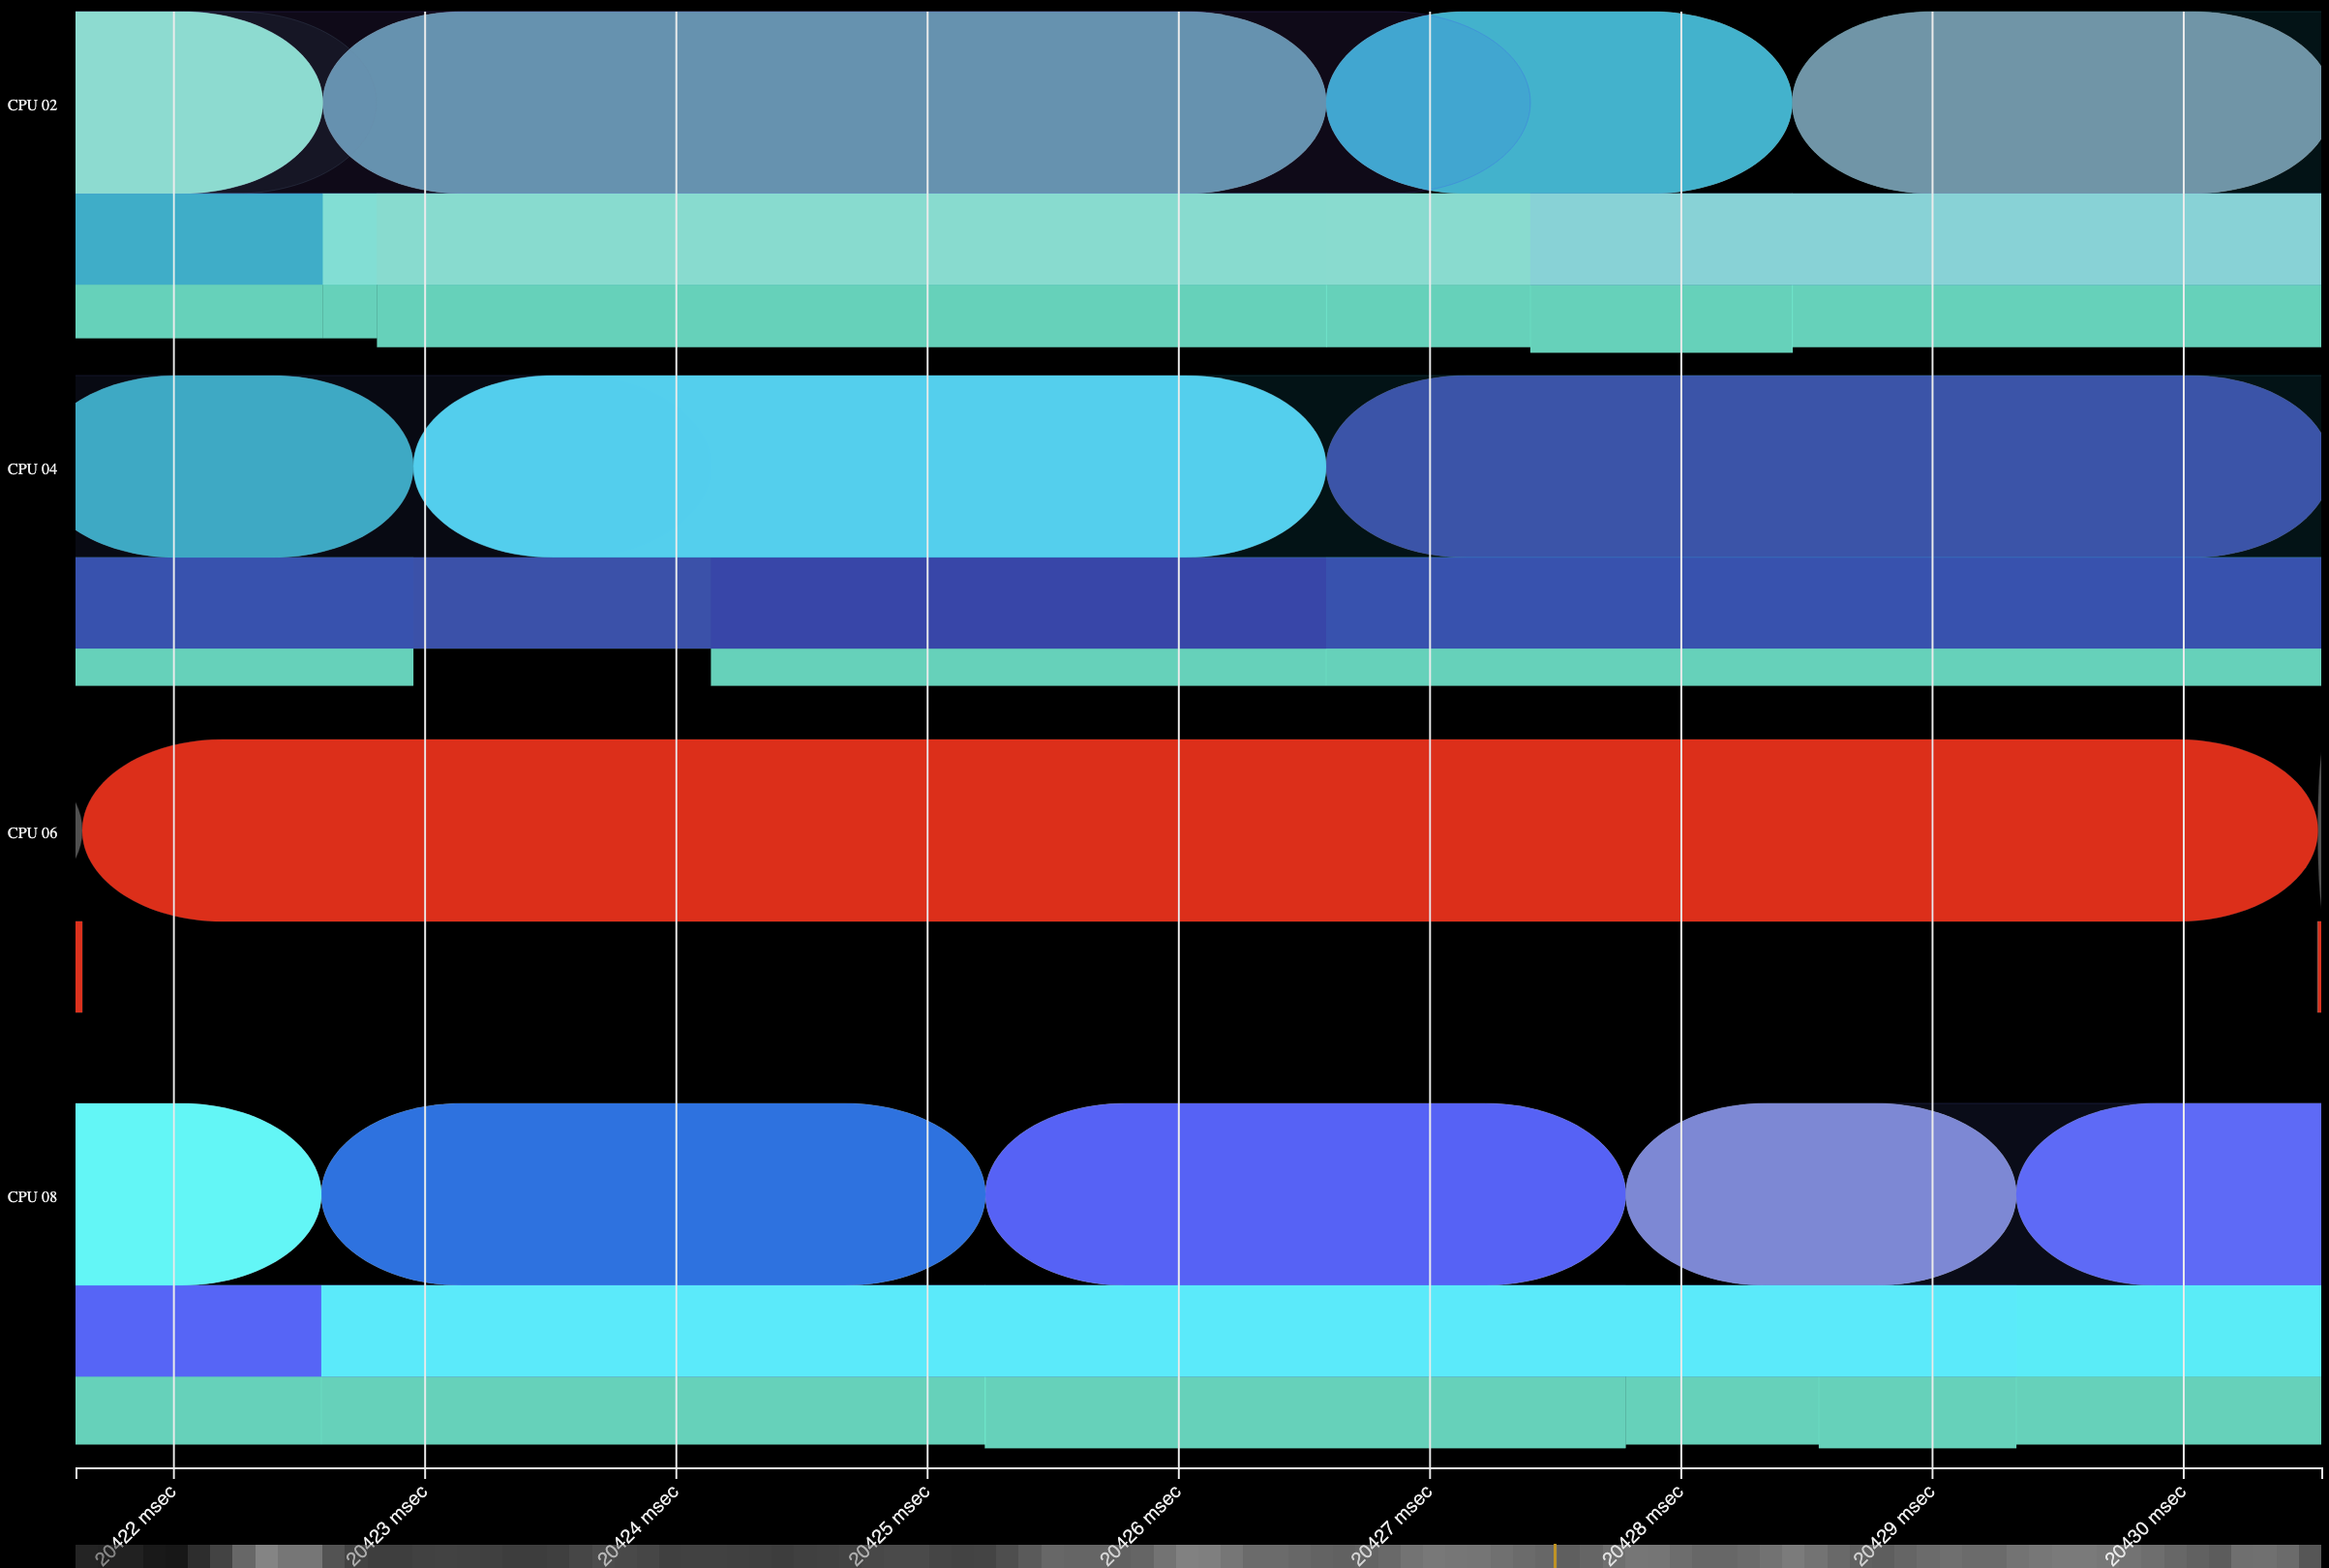
\includegraphics[width=\columnwidth]{graphs/schedviz-problem.png}
    \caption{Core 6 runs an image resize process, unaware that the other cores
    have queued server threads}\label{fig:schedviz-problem}
\end{figure}

The latency impact on the LC happens because the BE occasionally runs
uncontended on one core, while another has queued server threads.
\autoref{fig:schedviz-problem} shows this happening in the trace: on core 6, the
red process running for 10ms is a BE thread, while server threads, in shades of
blue, are queued on the other cores.

This priority inversion happens because weights are only enforced within
runqueues, which are per-CPU. Although load balancing eventually remedies this,
it runs less frequently than scheduling does. For workloads with request
processing times in the millisecond range, waiting for the load balancer to run
influences final processing times.

In order to globally enforce weights, each scheduling decision would require a
search of all runqueues for potentially higher-weight processes, which is too
costly. 




